\documentclass{article}
\usepackage{amsfonts}
\usepackage{amsmath}
\usepackage{mathtools}
\usepackage{systeme}
\usepackage{polynom}
\usepackage{pgfplots}
\usepackage[shortlabels]{enumitem}
\everymath{\displaystyle}
\DeclarePairedDelimiter\ceil{\lceil}{\rceil}
\newcommand{\p}[1]{\frac{\partial}{\partial #1}}
\begin{document}
\begin{center}
\Large\textbf{Kodutöö nr. 4}\\
1. variant\\
\small{Joosep Näks}
\end{center}
\textbf{1. }Tõestada, et kui $D\subset \mathbb{R}$ on Jordani mõttes mõõtuv mittetühi hulk, kusjuures $D\subset \overline{D^\circ}$, siis hulga $D$ Jordani mõõt $\mu(D)>0$.\\\\
\textbf{Lahendus:}\\
On teada, et hulgal $D$ leidub sisepunkte, kuna kui ei leiduks, oleks $D^\circ$ tühihulk ehk ka $\overline{D^\circ}$ oleks tühihulk, ehk $D$ oleks tühihulga osahulk ehk tühihulk, kuid on teada, et $D$ on mittetühi.\\
Definitsiooni järgi kui punkt $x$ on hulga $D$ sisepunkt, siis leidub tal ümbrus $U_\varepsilon$, mis on $D$ osahulk. Ümbruse mõõt reaalteljel on $\mu(U_\varepsilon)=2\varepsilon$ ning kuna see on $D$ osahulk, siis $\mu(D)\geq\mu(U_\varepsilon)>0$.\\\\\\\\
\textbf{2.} Leida sellise keha ruumala, mis on piiratud silindriga $x^2+y^2=2x$ ja koonusega $z^2=x^2+y^2$.\\\\
\textbf{Lahendus:}\\
Teisendades võrrandit $x^2+y^2=2x$ saan $(x-1)^2+y^2=1$ ehk see joon piirab $\mathbb{R}^2$ tasandil kera $B((1,0),1)$.\\
Avaldan koonuse võrrandist $z$:$$z=\pm\sqrt{x^2+y^2}$$Siit saan kaks funktsiooni, $f(x,y)=\sqrt{x^2+y^2}$ ja $g(x,y)=-\sqrt{x^2+y^2}$. Kuna ruutjuur annab reaalarvuliste väärtuste korral positiivseid väärtuseid, kehtib $f(x,y)\geq g(x,y)$.\\
Seega on täidetud loengukonspekti teoreemi 6.2 eeldused ning ruumala on võrdne integraaliga $$\iint\limits_{B((0,1),1)}(f(x,y)-g(x,y))dx\ dy=\iint\limits_{B((0,1),1)}2\sqrt{x^2+y^2}dx\ dy$$Integraali leidmiseks teen ülemineku polaarkoordinaatidesse teisednusega $x=r\cos\phi,\ y=r\sin\phi$. Integreeritavasse funktsiooni teisenduse sisse asendades saan $2\sqrt{x^2+y^2}=2r$ ning kuna teisenduse jakobiaan on $r$, korrutan funktsiooni sellega läbi.\\
 Loon joonise silindri projektsioonist $xy$ tasandile.
\begin{center}
\begin{tikzpicture}
\begin{axis}[domain=-0.3:2.2,
             axis lines=middle,
    grid style=dashed,]
        \addplot[color=blue,samples=500] {(1-(\x-1)^2)^0.5};
        \addplot[color=blue,samples=500] {-(1-(\x-1)^2)^0.5};
\addlegendentry{$(x-1)^2+y^2=1$}
        
\end{axis}
\end{tikzpicture}
\end{center}
Siit on näha, et $\phi$ rajad on $-\frac{\pi}2$ ja $\frac{\pi}2$. $r$ alumine raja on 0, ülemise raja leidmiseks asendan teisenduse silindri võrrandisse: $x^2+y^2=2x \Leftrightarrow r^2=2r\cos\phi\Leftrightarrow r=2\cos\phi$. Seega saan integraali:
\begin{gather*}
\begin{aligned}
\iint\limits_E 2\sqrt{x^2+y^2}dx\ dy=&\int_{-\frac{\pi}2}^\frac{\pi}2\int_0^{2\cos\phi}2r^2dr\ d\phi\\
=&\int_{-\frac{\pi}2}^\frac{\pi}2(\frac{2r^3}{3})\bigg|_0^{2\cos\phi\ d\phi}\\
=&\frac23\int_{-\frac{\pi}2}^\frac{\pi}2(2\cos\phi)^3\ d\phi\\
=&\frac{16}3\int_{-\frac{\pi}2}^{\frac{\pi}2}(1-\sin^2\phi)\cos\phi\ d\phi\\
=&\frac{16}3\int_{-\frac{\pi}2}^{\frac{\pi}2}(1-\sin^2\phi)\ d(\sin\phi)\\
=&\frac{16}3\cdot\left(\sin\phi-\frac{\sin^3\phi}3\right)\bigg|_{-\frac{\pi}2}^{\frac{\pi}2}\\
=&\frac{16}32\left(1-\frac13\right)\\
=&\frac{64}{9}
\end{aligned}
\end{gather*}
\pagebreak\\
\textbf{3. }Leida kolmekordne integraal $\iiint\limits_E z^2\ dx\ dy\ dz$, kui hulk $E$ on piiratud pindadega $$y=10x,\quad y=0,\quad x=1,\quad z=xy\quad \text{ja}\quad z=0.$$\\
\textbf{Lahendus:}\\
$z$ teljel on hulk $E$ piiratud ühelt poolt pinnaga $z=0$ ning teiselt poolt $z=xy$, seega võtan need sisemise integraali rajadeks. $y$ teljel on hulk piiratud ühelt poolt pinnaga $y=0$ ja teiselt poolt $y=10x$ seega võtan need rajadeks. Need pinnad puutuvad kokku $x$ väärtusel $x=0$, seega on see $x$ teljel alumine raja. Ülemine raja $x$ teljel on $x=1$.\\
Seega saan:
\begin{gather*}
\begin{aligned}
\iiint\limits_E z^2\ dx\ dy\ dz &= \int_0^1\int_0^{10x}\int_0^{xy}z^2\ dz\ dy\ dx\\
&=\int_0^1\int_0^{10x}\left(\left.\frac{z^3}{3}\right)\right|_0^{xy}\ dy\ dx\\
&=\int_0^1\int_0^{10x}\frac{(xy)^3}{3}\ dy\ dx\\
&=\int_0^1\left(\left.\frac{x^3y^4}{12}\right)\right|_0^{10x}\ dx\\
&=\int_0^1\frac{x^3(10x)^4}{12}\ dx\\
&=\frac{1000}{12}\int_0^1x^7\ dx\\
&=\frac{1000}{12}\left(\left.\frac{x^8}{8}\right)\right|_0^1\\
&=\frac{1000}{12}\cdot\frac{1}{8}\\
&=\frac{125}{12}\\
\end{aligned}
\end{gather*}
\pagebreak\\
\textbf{4. }Üleminekuga sfäärilistele koordinaatidele leida kolmekordne integraal $$\iiint\limits_E\frac{z^2\ dx\ dy\ dz}{x^2+y^2+z^2}$$ kui hulk $E$ on piiratud pinnaga $x^2+y^2+z^2=z$\\\\
\textbf{Lahendus:}\\
Teen ülemineku sfäärilistesse koordinaatidesse teisendusega $x=r\sin\theta\cos\phi,\ y=r\sin\theta\sin\phi,\ z=r\cos\theta$.\\
Leian sfääriliste koordinaatide rajad. Hulka $E$ piirav pind on teisendades $x^2+y^2+\left(z-\frac12\right)^2=\frac14$ ehk kera raadiusega $\frac12$ ja keskpunktiga $\left(0,0,\frac12\right)$. Seega asub see täielikult $z=0$ tasandist mitte madalamal $z$ telge pidi, ehk $\theta\in\left(0,\frac{\pi}2\right)$. $r$ alumine raja on 0 kuna kera puutub $(0,0,0)$ punkti ning ülemise raja leidmiseks asendan teisenduse $E$ piirava pinna võrrandisse ja saan $r=\cos\theta$.\\
Leian integreeritava funktsiooni. Asendades teisenduse algsesse integreeritavasse funktisooni sisse saan $$\frac{z^2}{x^2+y^2+z^2}=\frac{r^2\cos^2\theta}{r^2}=\cos^2\theta$$ ning kuna teisenduse jakobiaan on $r^2\sin\theta$, korrutan funktsiooni sellega läbi. Seega saan integraali:
\begin{gather*}
\begin{aligned}
\iiint\limits_E\frac{z^2\ dx\ dy\ dz}{x^2+y^2+z^2}=&\int_0^\frac{\pi}2\int_0^{2\pi}\int_0^{\cos\theta}r^2\cos^2\theta\sin\theta\ dr\ d\phi\ d\theta\\
=&\int_0^\frac{\pi}2\int_0^{2\pi}\cos^2\theta\sin\theta\frac{r^3}{3}\bigg|_0^{\cos\theta}\ d\phi\ d\theta\\
=&\int_0^\frac{\pi}2\int_0^{2\pi}\cos^2\theta\sin\theta\frac{\cos^3\theta}{3}\ d\phi\ d\theta\\
=&\int_0^\frac{\pi}2\sin\theta\frac{\cos^5\theta}{3}\phi\big|_0^{2\pi}\ d\theta\\
=&\int_0^\frac{\pi}2\sin\theta\frac{\cos^5\theta}{3}2\pi\ d\theta\\
=&\frac{2\pi}3\int_0^\frac{\pi}2\cos^5\theta\ d\cos\theta\\
=&\frac{2\pi}3\frac{\cos^6\theta}6\bigg|_0^\frac{\pi}2\\
=&\frac{\pi}9\\
\end{aligned}
\end{gather*}
\pagebreak\\
\textbf{5.} Kolmekordse integraali abil leida keha $E$ ruumala, kui keha $E$ on piiratud pindadega $$x^2+y^2=x,\quad y=0,\quad y=x,\quad z=0\quad\text{ja}\quad z=\sqrt{x^2+y^2} $$Kolmekordse integraali arvutamisel minna üle silindrilistele koordinaatidele.\\\\
\textbf{Lahendus:}\\
Keha $E$ ruumala saab leida integraaliga $\iiint\limits_E dx\ dy\ dz$. Esimesed kolm pinda on $xy$ tasandiga risti ja moodustavad sellel järgneva joonise: 
\begin{center}
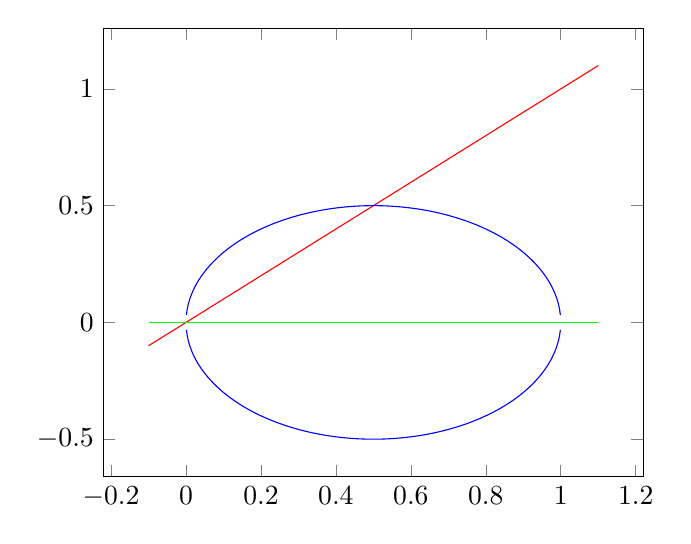
\begin{tikzpicture}
\begin{axis}[domain=-0.1:1.1]
        \addplot[color=red] {\x};
        \addplot[color=blue,samples=500] {(1/4-(\x-1/2)^2)^0.5};
        \addplot[color=blue,samples=500] {-(1/4-(\x-1/2)^2)^0.5};
        \addplot[color=green] {0};
\end{axis}
\end{tikzpicture}
\end{center}
Seega on keha $E$ kõversilinder, mille põhja pind on $$\{(x,y)\ |\ 0<x<\frac{1}{2},0<y<x\}\cup\left\{(x,y)\ \Big|\ \frac{1}{2}<x<1,0<y<\sqrt{\frac14-\left(x-\frac12\right)^2}\right\}.$$Minnes üle silindrililistesse koordinaatidesse teisendusega $$x=r\cos\phi,\quad y=r\sin\phi,\quad z=h$$ $r$ ülemiseks piiriks saab koosinusteoreemist $\sqrt{\frac12-\frac{\cos(\pi-2\phi)}2}$, millest saab lihtsustades $\cos\phi$. Jooniselt on näha, et nurk $\phi$ liigub pindade $y=0$ ja $y=x$ vahel ehk $\phi\in\left[0,\frac{\pi}4\right]$.\\Seega saan integraali
\begin{gather*}
\begin{aligned}
\iiint\limits_E dx\ dy\ dz=&\int_0^{\frac{\pi}4}\int_0^{\cos\phi}\int_0^rr\ dh\ dr\ d\phi\\
=&\int_0^{\frac{\pi}4}\int_0^{\cos\phi}\left(rh\right)\big|_0^r\ dr\ d\phi\\
=&\int_0^{\frac{\pi}4}\int_0^{\cos\phi}r^2\ dr\ d\phi\\
=&\int_0^{\frac{\pi}4}\left(\frac{r^3}3\right)\bigg|_0^{\cos\phi}\ d\phi\\
=&\int_0^{\frac{\pi}4}\frac{\cos^3\phi}3\ d\phi\\
=&\int_0^{\frac{\pi}4}\frac{(1-\sin^2\phi)\cos\phi}3\ d\phi\\
=&\int_0^{\frac{\pi}4}\frac{1-\sin^2\phi}3\ d(\sin\phi)\\
=&\frac{\sin\phi-\frac{\sin^3\phi}3}3\bigg|_0^{\frac{\pi}4}\\
=&\frac{\frac1{\sqrt{2}}-\frac{1}{6\sqrt{2}}}3\\
=&\frac{5}{18\sqrt{2}}\\
\end{aligned}
\end{gather*} 
\end{document}